\pdfoutput=1
% ---------------------------------------------------------------------------
% What extraction cannot slim, and whether function injection can.
% A pre-registered count of the long methods in 580 open-source Java
% repositories, as they stood before AI coding assistants.
%
% Built for arXiv (primary class cs.SE). No .bib: the bibliography is a
% `thebibliography` environment at the end.
%
% Every number in this file is a macro from generated/numbers.tex and every
% table is a fragment under generated/, both written by paper/scripts/numbers.py
% from results/analysis/analysis.json (the registered analysis, step 4) and
% results/analysis/posthoc.json (the post hoc readings, step 5). No number is
% typed by hand: the plan's own constants and what the plan records as seen
% before registration also come through the script. The only exceptions are
% the plan's own dates in the Introduction and the registration commit below;
% a reader checks the commit in the public repository, or reruns the steps.
% Code, files and commands are named in the ancillary README, not here.
%
% Build:   pdflatex main && pdflatex main
% ---------------------------------------------------------------------------
\documentclass[11pt,a4paper]{article}

\usepackage[T1]{fontenc}
\usepackage[utf8]{inputenc}
\usepackage{lmodern}
\usepackage[margin=2.4cm]{geometry}
\usepackage{graphicx}
\usepackage{booktabs}
\usepackage{array}
\usepackage{multirow}
\usepackage{amsmath}
\usepackage{tikz}
\usepackage{microtype}
\usepackage[hidelinks]{hyperref}
\hypersetup{pdftitle={What extraction cannot slim, and whether function injection can: a pre-registered count of the long methods in 580 open-source Java repositories},
  pdfauthor={Daniel Sagenschneider}, pdfsubject={Software engineering: empirical study of long-method refactoring}}
\usepackage{caption}
\captionsetup{font=small,labelfont=bf}

% Written by paper/scripts/numbers.py from results/analysis/analysis.json, posthoc.json and exploratory/results/explore.json. Do not edit.
\newcommand{\nDrawn}{757}
\newcommand{\nUsable}{580}
\newcommand{\nExcluded}{177}
\newcommand{\nError}{0}
\newcommand{\nScanned}{580}
\newcommand{\nNotScanned}{0}
\newcommand{\popHigh}{546}
\newcommand{\usableHigh}{224}
\newcommand{\weightHigh}{2.4}
\newcommand{\popMid}{2{,}539}
\newcommand{\usableMid}{191}
\newcommand{\weightMid}{13.3}
\newcommand{\popLow}{8{,}818}
\newcommand{\usableLow}{165}
\newcommand{\weightLow}{53.4}
\newcommand{\sampleFracHigh}{46\%}
\newcommand{\nMethods}{3{,}026{,}902}
\newcommand{\nLong}{168{,}466}
\newcommand{\longShare}{5.6\%}
\newcommand{\nUnparsed}{173}
\newcommand{\nSlimmable}{105{,}869}
\newcommand{\nLocked}{24{,}164}
\newcommand{\nRecord}{3{,}727}
\newcommand{\nNotSlimmable}{34{,}706}
\newcommand{\nSlims}{130{,}033}
\newcommand{\slimsShare}{77.2\%}
\newcommand{\nStuck}{38{,}433}
\newcommand{\stuckShare}{22.8\%}
\newcommand{\recordShareOfStuck}{9.7\%}
\newcommand{\slimCostMedian}{3}
\newcommand{\slimCostQone}{2}
\newcommand{\slimCostQthree}{6}
\newcommand{\slimCostMax}{199}
\newcommand{\nStuckPlanned}{21{,}329}
\newcommand{\ofStuckPlanned}{38{,}433}
\newcommand{\pooledStuckPlanned}{55.5\%}
\newcommand{\popStuckPlanned}{55.5\%}
\newcommand{\loStuckPlanned}{52.0}
\newcommand{\hiStuckPlanned}{59.0}
\newcommand{\sampleLoStuckPlanned}{53.5}
\newcommand{\sampleHiStuckPlanned}{57.5}
\newcommand{\medianStuckPlanned}{60.0\%}
\newcommand{\reposStuckPlanned}{470}
\newcommand{\ciStuckPlanned}{55.5\% (95\% CI 52.0 to 59.0)}
\newcommand{\tierHighStuckPlanned}{55.5\%}
\newcommand{\tierMidStuckPlanned}{55.5\%}
\newcommand{\tierLowStuckPlanned}{55.4\%}
\newcommand{\nCatThree}{7{,}515}
\newcommand{\ofCatThree}{38{,}433}
\newcommand{\pooledCatThree}{19.6\%}
\newcommand{\popCatThree}{19.2\%}
\newcommand{\loCatThree}{17.5}
\newcommand{\hiCatThree}{21.3}
\newcommand{\sampleLoCatThree}{18.2}
\newcommand{\sampleHiCatThree}{21.2}
\newcommand{\medianCatThree}{14.5\%}
\newcommand{\reposCatThree}{470}
\newcommand{\ciCatThree}{19.2\% (95\% CI 17.5 to 21.3)}
\newcommand{\tierHighCatThree}{20.1\%}
\newcommand{\tierMidCatThree}{19.1\%}
\newcommand{\tierLowCatThree}{19.2\%}
\newcommand{\nStuckPlannedC}{24{,}327}
\newcommand{\ofStuckPlannedC}{38{,}433}
\newcommand{\pooledStuckPlannedC}{63.3\%}
\newcommand{\popStuckPlannedC}{63.3\%}
\newcommand{\loStuckPlannedC}{60.1}
\newcommand{\hiStuckPlannedC}{66.5}
\newcommand{\sampleLoStuckPlannedC}{61.4}
\newcommand{\sampleHiStuckPlannedC}{65.1}
\newcommand{\medianStuckPlannedC}{66.7\%}
\newcommand{\reposStuckPlannedC}{470}
\newcommand{\ciStuckPlannedC}{63.3\% (95\% CI 60.1 to 66.5)}
\newcommand{\tierHighStuckPlannedC}{63.4\%}
\newcommand{\tierMidStuckPlannedC}{63.1\%}
\newcommand{\tierLowStuckPlannedC}{63.4\%}
\newcommand{\nCatThreeC}{8{,}524}
\newcommand{\ofCatThreeC}{38{,}433}
\newcommand{\pooledCatThreeC}{22.2\%}
\newcommand{\popCatThreeC}{22.2\%}
\newcommand{\loCatThreeC}{20.3}
\newcommand{\hiCatThreeC}{24.3}
\newcommand{\sampleLoCatThreeC}{20.8}
\newcommand{\sampleHiCatThreeC}{23.8}
\newcommand{\medianCatThreeC}{17.4\%}
\newcommand{\reposCatThreeC}{470}
\newcommand{\ciCatThreeC}{22.2\% (95\% CI 20.3 to 24.3)}
\newcommand{\tierHighCatThreeC}{22.6\%}
\newcommand{\tierMidCatThreeC}{21.5\%}
\newcommand{\tierLowCatThreeC}{22.4\%}
\newcommand{\nImproved}{35{,}618}
\newcommand{\ofImproved}{130{,}033}
\newcommand{\pooledImproved}{27.4\%}
\newcommand{\popImproved}{29.0\%}
\newcommand{\loImproved}{24.3}
\newcommand{\hiImproved}{34.6}
\newcommand{\sampleLoImproved}{25.3}
\newcommand{\sampleHiImproved}{30.0}
\newcommand{\medianImproved}{21.5\%}
\newcommand{\reposImproved}{559}
\newcommand{\ciImproved}{29.0\% (95\% CI 24.3 to 34.6)}
\newcommand{\tierHighImproved}{27.1\%}
\newcommand{\tierMidImproved}{25.8\%}
\newcommand{\tierLowImproved}{30.2\%}
\newcommand{\nTied}{26{,}056}
\newcommand{\ofTied}{130{,}033}
\newcommand{\pooledTied}{20.0\%}
\newcommand{\popTied}{20.9\%}
\newcommand{\loTied}{19.1}
\newcommand{\hiTied}{23.0}
\newcommand{\sampleLoTied}{19.2}
\newcommand{\sampleHiTied}{21.1}
\newcommand{\medianTied}{19.1\%}
\newcommand{\reposTied}{559}
\newcommand{\ciTied}{20.9\% (95\% CI 19.1 to 23.0)}
\newcommand{\tierHighTied}{20.2\%}
\newcommand{\tierMidTied}{18.6\%}
\newcommand{\tierLowTied}{21.9\%}
\newcommand{\hOneReading}{refuted}
\newcommand{\hTwoReading}{estimate}
\newcommand{\hOneBar}{25\%}
\newcommand{\hOneMinimum}{30}
\newcommand{\tierMedianHighCatThreeC}{17.0\%}
\newcommand{\tierMedianMidCatThreeC}{15.8\%}
\newcommand{\tierMedianLowCatThreeC}{19.7\%}
\newcommand{\tierMedianHighStuckPlannedC}{68.0\%}
\newcommand{\tierMedianMidStuckPlannedC}{66.7\%}
\newcommand{\tierMedianLowStuckPlannedC}{69.9\%}
\newcommand{\tierMedianHighImproved}{24.2\%}
\newcommand{\tierMedianMidImproved}{20.3\%}
\newcommand{\tierMedianLowImproved}{20.0\%}
\newcommand{\catOne}{17{,}123}
\newcommand{\catOneC}{17{,}123}
\newcommand{\catOneShare}{44.6\%}
\newcommand{\catOneCShare}{44.6\%}
\newcommand{\catTwo}{3{,}727}
\newcommand{\catTwoC}{3{,}727}
\newcommand{\catTwoShare}{9.7\%}
\newcommand{\catTwoCShare}{9.7\%}
\newcommand{\catThree}{7{,}515}
\newcommand{\catThreeC}{8{,}524}
\newcommand{\catThreeShare}{19.6\%}
\newcommand{\catThreeCShare}{22.2\%}
\newcommand{\catFour}{10{,}068}
\newcommand{\catFourC}{9{,}059}
\newcommand{\catFourShare}{26.2\%}
\newcommand{\catFourCShare}{23.6\%}
\newcommand{\catThreeGain}{1{,}009}
\newcommand{\catThreeGainReasons}{a loop (647), carried values (300), a try (181), a long statement (58), a switch (11), a jump (1)}
\newcommand{\nStuckPlannedGain}{2{,}998}
\newcommand{\catOneTwoShare}{54.3\%}
\newcommand{\plannedButConventional}{15{,}803}
\newcommand{\plannedButConventionalShare}{65.0\%}
\newcommand{\nStuckNoPlan}{17{,}104}
\newcommand{\nLongNoPlan}{37{,}734}
\newcommand{\nStuckNoPlanC}{14{,}106}
\newcommand{\nLongNoPlanC}{14{,}122}
\newcommand{\loopShareStuckNoPlan}{48.3\%}
\newcommand{\loopShareStuckNoPlanC}{43.5\%}
\newcommand{\jumpsStuckNoPlan}{177}
\newcommand{\jumpsStuckNoPlanC}{484}
\newcommand{\nLongPlanC}{154{,}344}
\newcommand{\nInjectionUsed}{85{,}999}
\newcommand{\nExtractionOnly}{68{,}345}
\newcommand{\injectionUsedShareOfPlans}{55.7\%}
\newcommand{\nBoth}{111{,}583}
\newcommand{\splitSmallerSeam}{63.3\%}
\newcommand{\equalSeam}{32.2\%}
\newcommand{\splitLargerSeam}{4.5\%}
\newcommand{\medianSinewSeam}{2}
\newcommand{\medianSplitSeam}{1}
\newcommand{\splitSmallerParts}{5.6\%}
\newcommand{\equalParts}{27.6\%}
\newcommand{\splitLargerParts}{66.8\%}
\newcommand{\medianSinewParts}{1}
\newcommand{\medianSplitParts}{2}
\newcommand{\splitSmallerLargest}{8.4\%}
\newcommand{\equalLargest}{24.8\%}
\newcommand{\splitLargerLargest}{66.8\%}
\newcommand{\medianSinewLargest}{16}
\newcommand{\medianSplitLargest}{24}
\newcommand{\nWorse}{4{,}993}
\newcommand{\worseByOne}{4{,}197}
\newcommand{\worseByOneShare}{84.1\%}
\newcommand{\worseByTwo}{650}
\newcommand{\worseByThreePlus}{146}
\newcommand{\worseMax}{5}
\newcommand{\nTiedK}{26{,}056}
\newcommand{\notImprovedShare}{52.6\%}
\newcommand{\nNotImproved}{68{,}359}
\newcommand{\savingMedian}{2}
\newcommand{\savingQone}{1}
\newcommand{\savingQthree}{4}
\newcommand{\savingMean}{3.4}
\newcommand{\savingMax}{50}
\newcommand{\savingOneShare}{39.2\%}
\newcommand{\nImprovedStrict}{21{,}655}
\newcommand{\pooledImprovedStrict}{16.7\%}
\newcommand{\popImprovedStrict}{17.2\%}
\newcommand{\loImprovedStrict}{14.6}
\newcommand{\hiImprovedStrict}{20.1}
\newcommand{\ciImprovedStrict}{17.2\% (95\% CI 14.6 to 20.1)}
\newcommand{\medianImprovedStrict}{11.9\%}
\newcommand{\improvedFunctionsOnly}{25{,}188}
\newcommand{\improvedWithPieces}{10{,}430}
\newcommand{\improvedWithPiecesShare}{29.3\%}
\newcommand{\catThreeCFunctionsOnly}{5{,}514}
\newcommand{\catThreeCWithPieces}{3{,}010}
\newcommand{\catThreeCWithPiecesShare}{35.3\%}
\newcommand{\topTenShare}{38.0\%}
\newcommand{\topThirtyShare}{57.8\%}
\newcommand{\topRepo}{corretto/\allowbreak corretto-8}
\newcommand{\topRepoStuck}{4{,}384}
\newcommand{\topRepoStuckShare}{11.4\%}
\newcommand{\topRepoCatThreeC}{889}
\newcommand{\topRepoCatThreeCShare}{20.3\%}
\newcommand{\topTenCatThreeCMin}{16.9\%}
\newcommand{\topTenCatThreeCMax}{33.9\%}
\newcommand{\reposNoLong}{18}
\newcommand{\reposNoStuck}{110}
\newcommand{\reposStuckNoCatThree}{124}
\newcommand{\medianLongPerRepo}{42.5}
\newcommand{\medianStuckPerRepo}{7}
\newcommand{\catThreeCQone}{0.0\%}
\newcommand{\catThreeCQthree}{28.8\%}
\newcommand{\reposStuckNoCatThreeShare}{26.4\%}
\newcommand{\machineLines}{500}
\newcommand{\catFourGui}{48}
\newcommand{\catFourLongTable}{130}
\newcommand{\catFourMachine}{176}
\newcommand{\catFourMachineShare}{1.9\%}
\newcommand{\testDroppedLong}{8{,}191}
\newcommand{\testDroppedLongShare}{4.9\%}
\newcommand{\testDroppedStuck}{1{,}007}
\newcommand{\testDroppedCatThreeC}{99}
\newcommand{\testDroppedCatThreeCShare}{9.8\%}
\newcommand{\testRepos}{80}
\newcommand{\testTopSegment}{test-applications}
\newcommand{\testTopSegmentCount}{2{,}900}
\newcommand{\testSecondSegment}{internalClusterTest}
\newcommand{\testSecondSegmentCount}{1{,}772}
\newcommand{\testHOnePop}{22.7\%}
\newcommand{\testHOneLo}{21.0}
\newcommand{\testHOneHi}{24.7}
\newcommand{\testHOneReading}{refuted}
\newcommand{\testHTwoPop}{29.5\%}
\newcommand{\testHTwoLo}{24.8}
\newcommand{\testHTwoHi}{35.1}
\newcommand{\testHOneCi}{22.7\% (95\% CI 21.0 to 24.7)}
\newcommand{\testHTwoCi}{29.5\% (95\% CI 24.8 to 35.1)}
\newcommand{\planInCatOne}{13{,}012}
\newcommand{\planInCatOneShare}{76.0\%}
\newcommand{\planInCatTwo}{2{,}791}
\newcommand{\planInCatTwoShare}{74.9\%}
\newcommand{\planInCatThree}{7{,}326}
\newcommand{\planInCatThreeShare}{97.5\%}
\newcommand{\planInCatFour}{1{,}198}
\newcommand{\planInCatFourShare}{11.9\%}
\newcommand{\nNotConventional}{17{,}583}
\newcommand{\rescueOfNotConventional}{48.5\%}
\newcommand{\rescueOfNotConventionalPop}{47.2\%}
\newcommand{\rescueOfNotConventionalLo}{43.4}
\newcommand{\rescueOfNotConventionalHi}{51.2}
\newcommand{\rescueOfNotConventionalMedian}{50.0\%}
\newcommand{\rescueOfNotConventionalCi}{47.2\% (95\% CI 43.4 to 51.2)}
\newcommand{\nCatThreeLost}{189}
\newcommand{\nCatThreeLostJumps}{189}
\newcommand{\shapeNImproved}{35{,}618}
\newcommand{\shapeImprovedSequence}{79.3\%}
\newcommand{\shapeImprovedSequenceReturns}{17.1\%}
\newcommand{\shapeImprovedBranching}{3.0\%}
\newcommand{\shapeImprovedBranchingReturns}{0.6\%}
\newcommand{\shapeImprovedAnySequence}{96.4\%}
\newcommand{\shapeImprovedAnyBranching}{3.6\%}
\newcommand{\shapeNTied}{26{,}056}
\newcommand{\shapeTiedSequence}{83.1\%}
\newcommand{\shapeTiedSequenceReturns}{14.6\%}
\newcommand{\shapeTiedBranching}{2.2\%}
\newcommand{\shapeTiedBranchingReturns}{0.2\%}
\newcommand{\shapeTiedAnySequence}{97.7\%}
\newcommand{\shapeTiedAnyBranching}{2.3\%}
\newcommand{\shapeNRescued}{8{,}524}
\newcommand{\shapeRescuedSequence}{25.7\%}
\newcommand{\shapeRescuedSequenceReturns}{10.0\%}
\newcommand{\shapeRescuedBranching}{45.2\%}
\newcommand{\shapeRescuedBranchingReturns}{19.2\%}
\newcommand{\shapeRescuedAnySequence}{35.7\%}
\newcommand{\shapeRescuedAnyBranching}{64.3\%}
\newcommand{\shapeRescuedReturnsOfBranching}{29.8\%}
\newcommand{\nSeqWay}{37{,}381}
\newcommand{\popSeqWay}{23.8\%}
\newcommand{\ciSeqWay}{23.8\% (95\% CI 19.2 to 29.8)}
\newcommand{\nSeqWayStrict}{23{,}763}
\newcommand{\popSeqWayStrict}{14.8\%}
\newcommand{\ciSeqWayStrict}{14.8\% (95\% CI 12.2 to 18.0)}
\newcommand{\nSeqWayTied}{62{,}832}
\newcommand{\popSeqWayTied}{39.8\%}
\newcommand{\ciSeqWayTied}{39.8\% (95\% CI 33.6 to 48.5)}
\newcommand{\nInjWay}{44{,}142}
\newcommand{\popInjWay}{27.5\%}
\newcommand{\ciInjWay}{27.5\% (95\% CI 23.5 to 32.6)}
\newcommand{\nSeqImproved}{34{,}340}
\newcommand{\popSeqImproved}{22.0\%}
\newcommand{\ciSeqImproved}{22.0\% (95\% CI 17.5 to 28.2)}
\newcommand{\nSeqRescued}{3{,}041}
\newcommand{\popSeqRescued}{1.7\%}
\newcommand{\ciSeqRescued}{1.7\% (95\% CI 1.4 to 2.1)}
\newcommand{\nSeqWayMethods}{37{,}381}
\newcommand{\popSeqWayMethods}{1.5\%}
\newcommand{\ciSeqWayMethods}{1.5\% (95\% CI 1.1 to 2.1)}
\newcommand{\nExceptions}{16}
\newcommand{\nExceptionsJumps}{14}
\newcommand{\nExceptionsLongStatement}{2}
\newcommand{\exceptionsShare}{0.012\%}
\newcommand{\longConventional}{165{,}099}
\newcommand{\longEntryPoint}{3{,}190}
\newcommand{\longOfficeFloor}{177}
\newcommand{\allOfficeFloor}{835}
\newcommand{\allEntryPoint}{50{,}057}
\newcommand{\ofTopRepo}{geonetwork/\allowbreak core-geonetwork}
\newcommand{\ofTopRepoCount}{123}
\newcommand{\ofTopEvidence}{@Parameter}
\newcommand{\unparsedTopRepo}{alibaba/\allowbreak COLA}
\newcommand{\unparsedTopRepoCount}{65}
\newcommand{\unparsedSecondRepo}{java110/\allowbreak MicroCommunity}
\newcommand{\unparsedSecondRepoCount}{44}
\newcommand{\scanTotalMinutes}{121~min}
\newcommand{\scanMedianSeconds}{3.6}
\newcommand{\scanLongestRepo}{OpenLiberty/\allowbreak open-liberty}
\newcommand{\scanLongestMinutes}{38~min}
\newcommand{\scanWallHours}{2~h~1~min}
\newcommand{\scanDate}{3 November 2026}
\newcommand{\longestMethodLines}{5{,}976}
\newcommand{\longestMethodRepo}{plantuml/\allowbreak plantuml}
\newcommand{\longestMethodName}{MapData()}
\newcommand{\planSeed}{20261101}
\newcommand{\planTarget}{580}
\newcommand{\planAsOf}{1 December 2020}
\newcommand{\planMinFunctions}{50}
\newcommand{\planMinFiles}{15}
\newcommand{\samplerVersion}{0.3.0}
\newcommand{\slimVersion}{0.5.2}
\newcommand{\slimSha}{513b669f61c7}
\newcommand{\planHOneShare}{25\%}
\newcommand{\planHOneMinimum}{30}
\newcommand{\planResamples}{10{,}000}
\newcommand{\planLevel}{95\%}
\newcommand{\priorStuck}{119}
\newcommand{\priorCatThree}{12}
\newcommand{\priorCatThreeShare}{10.1\%}
\newcommand{\priorSlimmed}{327}
\newcommand{\priorImproved}{95}
\newcommand{\priorImprovedShare}{29\%}
\newcommand{\priorTied}{59}
\newcommand{\amendScansThree}{69}
\newcommand{\amendScansFive}{469}
\newcommand{\amendDiffering}{2}
\newcommand{\amendRescanned}{150}
\newcommand{\amendSpot}{15}
\newcommand{\amendUncompared}{96}
\newcommand{\exTables}{3{,}030}
\newcommand{\exTablesShare}{33.4\%}
\newcommand{\exIndivisibleShare}{50.5\%}
\newcommand{\exDataShare}{35.7\%}
\newcommand{\exControlShare}{13.7\%}
\newcommand{\exControlContainedShare}{91\%}
\newcommand{\exRegrouped}{219}
\newcommand{\exLimitSix}{4.4\%}
\newcommand{\exLimitTen}{12.5\%}
\newcommand{\exRepos}{329}
\newcommand{\exHotRepos}{32}
\newcommand{\exHotShare}{40\%}
\newcommand{\exHotLongShare}{22\%}
\newcommand{\exCogCatFour}{46.2}
\newcommand{\exCogRescued}{45.9}
\newcommand{\exCogConventional}{59.6}


\newcommand{\fitwidth}[1]{\resizebox{\ifdim\width>\textwidth\textwidth\else\width\fi}{!}{#1}}
\newcommand{\sig}[1]{\texttt{#1}}
\newcommand{\Hone}{H1}
\newcommand{\Htwo}{H2}

\title{\bfseries What extraction cannot slim, and whether function injection can\\
A pre-registered count of the long methods in \nUsable{} open-source Java repositories, as they stood before AI coding assistants}

% Zenodo DOI, reserved before publishing and printed under the author block.
% \newcommand{\thedoi}{10.5281/zenodo.XXXXXXXX}
\newcommand{\doiline}{\ifdefined\thedoi\quad\small\texttt{doi:\thedoi}\fi}

% The registration: the commit of the study's public repository that set the plan.
\newcommand{\regCommit}{bcb5d48}

\author{Daniel Sagenschneider\\\small OfficeFloor\\\small\texttt{daniel@officefloor.net}\doiline}

\date{November 2026}

\begin{document}
\maketitle

\begin{abstract}
\noindent
A method of 26 code lines or more reads as a Long Method, and Extract Method
is the usual fix. For some long methods there is no single-exit fix: a return
cannot leave an extracted piece, a piece hands back one value, and some
methods are knotted so that every cut is blocked. Function injection, as the
OfficeFloor framework does it, cuts differently: each piece becomes a function
the framework injects and sequences, an early return ends a function, and a
function hands on several values. The author of that framework pre-registered
a test of whether it takes apart the methods extraction cannot, with the
hypotheses, the sample's seed and the reading rule committed before any
repository was scanned. A stratified random sample of \nUsable{} open-source
Java repositories, each pinned to its last commit before \planAsOf{}, was
scanned by released tools whose cost models were fixed before the plan:
\nMethods{} methods, \nLong{} of them long. Single-exit extraction, as
SinewSlim models it, slims \slimsShare{} of the long methods; \nStuck{}
are stuck. The registered hypothesis, that at least a quarter of the stuck
methods are ones only function injection takes apart, is refuted:
\ciCatThreeC{}. The split has a plan for \popStuckPlannedC{} of the stuck
methods; nearly half of the stuck methods are early-return methods the plan
counts as conventionally fixable, and the split takes three in four of those
apart as they stand. Where extraction would do, the split chooses injection
and costs less for \ciImproved{} against extraction wrapped as one function,
and for \popImprovedStrict{} against plain extraction; its plan is then a
straight sequence of functions in \shapeImprovedAnySequence{} of cases, a
pipeline, whose hand-offs the extraction cost model prices twice and the flow
cost model once. Where it rescues a stuck method, the plan branches in
\shapeRescuedAnyBranching{}. Every figure, every failure and every method where injection
does worse is reported.
\end{abstract}

\section{Introduction}

Fowler catalogued the Long Method and named its fix, Extract Method
\cite{fowler1999}. An earlier study of this author's found that the length at
which reviewers call a method a Long Method is 26 code lines, lines that hold
code with blank and comment lines not counted, and that nothing else they
could be judging beats that length \cite{longmethod}. A tool, SinewSlim,
followed: for every method of 26 lines or more it searches for the cheapest
set of extractions that brings the method, and every extracted piece, to 25
lines or fewer, pricing each cut by what crosses it. Tools that find Extract
Method opportunities are not new \cite{tsantalis2011, haas2016}; SinewSlim's
difference is that it prices every cut and says when no cut is feasible, and
that is where this paper starts. Some long methods cannot be slimmed by
extraction into single-exit pieces at all. A \sig{return} cannot leave such a
piece, so a method of guard clauses blocks every cut that contains one. An
extracted piece hands back one value, so a run of statements that produces
two needs a record to carry them, at a cost of its own. Some methods are
knotted so tightly that every cut needs more parameters than a reader should
follow. These methods are called \emph{stuck} here, and stuck means stuck
under extraction as SinewSlim models it: one exit, one output and at most five
parameters a piece.

Function injection cuts a method differently. In OfficeFloor, a framework the
author created, a function is an ordinary Java method whose arguments the
framework supplies, as dependency injection does \cite{fowler2004}, and whose
next function the framework chooses: the developer writes the pieces and the
wiring between them, and the framework sequences them. An early return
becomes the end of a function followed by a flow; an \sig{if} can become a
decision with a flow per branch; a function hands on several values, because
the next function asks the framework for them, and the instrument allows a
function five. So a method extraction cannot slim might still come apart as
functions. The author expected it would, often. That expectation is exactly
what a reader should not take on trust from the framework's author, and this
paper is the pre-registered test of it: the sample's seed, the hypotheses,
the bar and the rule for reading the result were committed before any
repository of the sample was read, every cost comes from released products
whose cost models were fixed before the plan, and every figure is reported
whichever way it points.

The test is read on code people wrote. Each repository of the sample is
pinned to its last commit before \planAsOf{}. That date is six months before
1 June 2021, which is itself before GitHub Copilot's technical preview of
29 June 2021 \cite{copilot2021}, so that no method in the sample was written
with the AI coding assistants that came into general use from then on. The
answer is a count: of \nLong{} long methods in \nUsable{} repositories,
\nStuck{} are stuck, and the split that function injection offers rescues
\popCatThreeC{} of them, under the quarter the plan set as the bar. The reach
is real, it is smaller than the author expected, and the rest of the paper
says what the stuck methods are instead.

\section{Background}

\paragraph{Extraction, and its cost.} SinewSlim reads a method's facts (its
statements, the values each declares, reads and writes, the jumps that leave
each run of statements) and searches for the segmentation into contiguous
runs whose extraction leaves every piece and the remainder at or under the
target. A run's \emph{seam} is what crosses its boundary, its inputs as
parameters and its output as a return value, at 1 each; a run is feasible
with at most one output, at most five inputs and no jump leaving it. The
search takes the segmentation with the smallest worst seam, then the fewest
pieces, then the smallest total. A method is \emph{slimmable} when one
exists; \emph{slimmable but locked} when every piece and the remainder are
bound to the class's fields or methods, so that a split moves nothing out of
the class; \emph{slimmable only with a record} when a piece must hand back
several values, at three per value; and \emph{not slimmable} otherwise, with
the obstacle named. The last two statuses are what this paper calls stuck.

\paragraph{The injection split.} OfficeFloorSlim, the second product, reads
the same facts and searches for a partition of the method's control flow into
functions, each at or under the target, with every line in some function. Its
cost model was decided before any of its figures was set beside SinewSlim's:
a value computed inside the method and carried to a later function costs 1
for each function that declares it, while values from outside the method,
its parameters and whatever the framework injects, are free; a function
costs 1 and a flow between functions costs 1; a function may carry at most
five values. A \sig{return} ends a function, a \sig{throw} becomes an
escalation, and an \sig{if} or \sig{switch} may become a decision whose
branches are flows. Loops, lambda bodies and labelled statements are never
cut between functions. Its worst seam is the most values any function
declares, the counterpart of SinewSlim's widest piece, with one difference
that matters for reading them side by side: SinewSlim's width prices the
method's own parameters when a piece reads them, and the split's seam does
not, since the framework injects them.

\paragraph{The combined split.} No OfficeFloor developer would wire a
ten-line calculation through the framework as functions and flows when
extracting a method would do. The combined split is what a developer would
do: functions where the flow divides, extracted methods inside them. Its
outer search is the injection split's; a function whose body is over the
target is allowed when SinewSlim's search, under its defaults, slims that
body as a method of its own. A body SinewSlim slims only with a record is
refused. The plan chosen is the one with the smallest \emph{sum} of the
injection total and SinewSlim's cost of the pieces inside the functions; on a
tie, the fewer pieces, then the fewer functions. The whole method as one
function, slimmed by SinewSlim, is always a candidate at SinewSlim's cost
plus 1, so wherever SinewSlim slims a method the combined split has a plan
and its sum is never more than SinewSlim's cost plus 1. That holds by
construction and is not a finding; a one-function plan is reported as
\emph{extraction only} and counted as SinewSlim's.

\paragraph{The categories.} A stuck method is put in one category, tested
conventional first, so that function injection is credited only with what
nothing simpler fixes: category 2 if a record slims it; else category 1 if
SinewSlim's defaults slim it once its jumps are ignored, the guard-clause
methods a developer could restructure; else category 3 if the OfficeFloor
column has a plan; else category 4, which needs a redesign. Category 3 is
the rescue, and the plan's hypothesis reads it under the combined split.

\paragraph{Related work.} Finding Extract Method opportunities is a settled
line of work. JDeodorant finds them by slicing \cite{tsantalis2011}, JExtract
by the dependencies among a method's statements \cite{silva2014}, SEMI by the
functional relevance of neighbouring statements \cite{charalampidou2017},
GEMS by a learned model \cite{xu2017}, and Haas and Hummel by a scored search
over long methods \cite{haas2016}. Maruyama's block-based slicing
\cite{maruyama2001} and Komondoor and Horwitz's semantics-preserving
extraction \cite{komondoor2000} take runs that are not contiguous or that
jump, which is where a single-exit piece fails; IDEs do the same for one
early return by handing back a flag the caller tests. Each of these proposes
cuts; none counts what no cut can do across a corpus, and that is the count
this paper makes, under one tool's rules. A length threshold for a long
method is usually a statistic over a corpus \cite{lanza2006}; the 26 used
here is what reviewers call long \cite{longmethod}. Function injection has
an older relative in flow-based programming \cite{morrison2010}, where a
program is a graph of processes passing packets along connections, and a
nearer one in dependency injection \cite{fowler2004}; what OfficeFloor adds
is that the pieces are methods of ordinary classes and the sequencing is the
framework's. The author knows of no prior count of how many long methods a
flow of functions can take apart that extraction cannot.

\paragraph{What was known before the plan.} The combined split had been run
on one repository, OfficeFloor's own, written by the author, before the
hypotheses were written: it rescued \priorCatThree{} of \priorStuck{} stuck
methods (\priorCatThreeShare{}), and of the \priorSlimmed{} long methods
SinewSlim slims it chose injection and cost less for \priorImproved{}
(\priorImprovedShare{}). That one repository pointed against the rescue
hypothesis. The plan records the author's expectation all the same: that
code written by many hands, before AI assistants, would show more methods
that only injection takes apart than the framework's own code does. The
\priorImprovedShare{} is why the second question has no threshold: a share
set after seeing it would test nothing.

\section{Method}

The analysis plan was registered on 1 November 2026 with every decision
settled, before the sample was drawn, by commit \sig{\regCommit} of the
study's public repository. Every change since is a dated amendment that
records what had been seen when it was made. The plan, the
pinned values, the step scripts and the amendments are in that repository,
named in the ancillary data. Everything below is as registered unless marked
post hoc.

\paragraph{The sample.} An independent tool, open-source-repository-sampler
\samplerVersion{}, drew a seeded, stratified simple random sample of GitHub
repositories with the plan's seed, \planSeed{}, chosen as one nobody had
drawn before; the study's scripts refuse any other seed. The frame is Java
repositories created before \planAsOf{} in three popularity tiers, high (over
5{,}000 stars), mid (1{,}000 to 5{,}000) and low (200 to 999), drawn equally.
Each repository is pinned to the newest commit on its default branch's
first-parent history committed before \planAsOf{}, and judged there: at least
\planMinFunctions{} functions in at least \planMinFiles{} files, repositories
owned by the author or by OfficeFloor excluded. Table~\ref{tab:sample} gives
each tier's population, what was drawn and what was usable; population
estimates weight each repository by its stratum's population over its usable
count. The draw finished on 2 November 2026 and is committed: \nDrawn{} drawn,
\nUsable{} usable, \nExcluded{} excluded by the criteria, \nError{} lost to
errors.

\begin{table}[t]
\centering\small
\caption{The sample: each tier's population before the as-of date, what was drawn, what met the criteria, and the stratum weight (population over usable) used for population estimates.}
\label{tab:sample}
\begin{tabular}{llrrrrr}
\toprule
Tier & Stars & Population & Drawn & Usable & Excluded & Weight \\
\midrule
High & over 5{,}000 & 546 & 253 & 224 & 29 & 2.4 \\
Mid & 1{,}000 to 5{,}000 & 2{,}539 & 252 & 191 & 61 & 13.3 \\
Low & 200 to 999 & 8{,}818 & 252 & 165 & 87 & 53.4 \\
\midrule
All & & 11{,}903 & 757 & 580 & 177 & \\
\bottomrule
\end{tabular}

\end{table}

\paragraph{The instruments.} Every cost comes from released products; the
study computes none. OfficeFloorSlim \slimVersion{}, built on SinewSlim
0.2.3, was run once per repository at its pinned commit, from a jar whose
digest is pinned in the study. It reports, for every long method, SinewSlim's
assessment under SinewSlim's defaults (trigger 26, target 25), the injection
split and the combined split, each with its plan or its reason for having
none, and the method's category under each. The scope is production Java:
every \sig{.java} file, leaving out \sig{src/test}, \sig{src/it}, build
output, generated directories and any directory named \sig{test} or
\sig{tests}.

\paragraph{The measures and the analysis.} Per repository and pooled, the
plan fixes the methods with a body and the long ones (L1), the long methods
by SinewSlim's status (L2) and their slim cost (L3), the stuck methods (S1)
and those each split has a plan for (S2, S2c), the stuck methods by category
under each split (S3, S3c), the worst seam, the number of parts and the
largest part side by side where both SinewSlim and the injection split have a
plan (C1, C2), the injection split's reasons where it has no plan (F1), and,
of the long methods SinewSlim slims, those where the combined split chooses
injection and its sum is below SinewSlim's cost plus 1 (\emph{improved}) or
equal to it (\emph{tied}), with the saving (K2). The two total costs are
never compared: they count different things, and the weight that would turn
one into the other is the very thing a sceptical reader would say was chosen
to favour function injection. The unit is the repository. Every interval is a
percentile bootstrap over repositories within strata, \planResamples{}
resamples with the plan's seed, at \planLevel{}; the bootstrap applies no
finite population correction, and the high tier's draw is \sampleFracHigh{}
of its population, so the intervals there are, if anything, wide. Each
headline figure is reported pooled, as a population estimate weighted by
stratum with its interval, per tier, and as the median of each repository's
own share, so that a few very large repositories cannot quietly carry a
pooled figure.

\paragraph{The hypotheses.} Each is read from the \planLevel{} interval of
its population estimate. \Hone{}, the rescue, is confirmatory: category 3
under the combined split is at least \planHOneShare{} of the stuck methods
and at least \planHOneMinimum{} methods, a bar fixed before any scan;
supported if the whole interval is at or above \planHOneShare{} and the count
reaches the minimum, refuted if the whole interval is below, inconclusive
otherwise. \Htwo{}, the improvement, is an estimate with no threshold: the
share of the long methods SinewSlim slims where the combined split chooses
injection and costs less; ties are reported beside it and never counted,
because the tie-break favours injection.

\paragraph{Amendments.} The instrument was re-pinned three times, each before
any figure of the plan's measures had been computed: twice for speed alone,
and once because the release the second amendment pinned changed
\amendDiffering{} of \amendScansFive{} compared results. The release used
gives the first registered release's results, so far as that was checked: of
the \nUsable{} scans, \amendScansFive{} were compared field for field with
the scans of the version before the fault, \amendScansThree{} of those with
the version first registered as well, and \amendSpot{} more were scanned by
both the version before the fault and the release used; all were equal, and
only equality was read. The other \amendUncompared{} repositories were never
scanned by an earlier version, since the earlier versions take hours on
them, and rest on the tests the amendments record. The plan's amendments
record each change and its evidence.

\section{Results}

Every usable repository was scanned (\nScanned{} of \nUsable{}, none
failed) on \scanDate{}; \nUnparsed{} files could not be parsed and were left
out. Figure~\ref{fig:flow} gives the whole count at a glance and
Table~\ref{tab:status} the corpus. Of \nMethods{} methods with a body,
\nLong{} (\longShare{}) are long. SinewSlim slims \nSlims{} of them
(\slimsShare{}) with one return per piece, at a median slim cost of
\slimCostMedian{} (quartiles \slimCostQone{} and \slimCostQthree{}), the
cost being SinewSlim's total for the whole segmentation rather than any one
seam. The rest, \nStuck{} (\stuckShare{}), are stuck: \nRecord{} slim only
with a record and \nNotSlimmable{} not at all. The shares are alike across
the tiers.

\begin{figure}[t]
\centering
\fitwidth{%
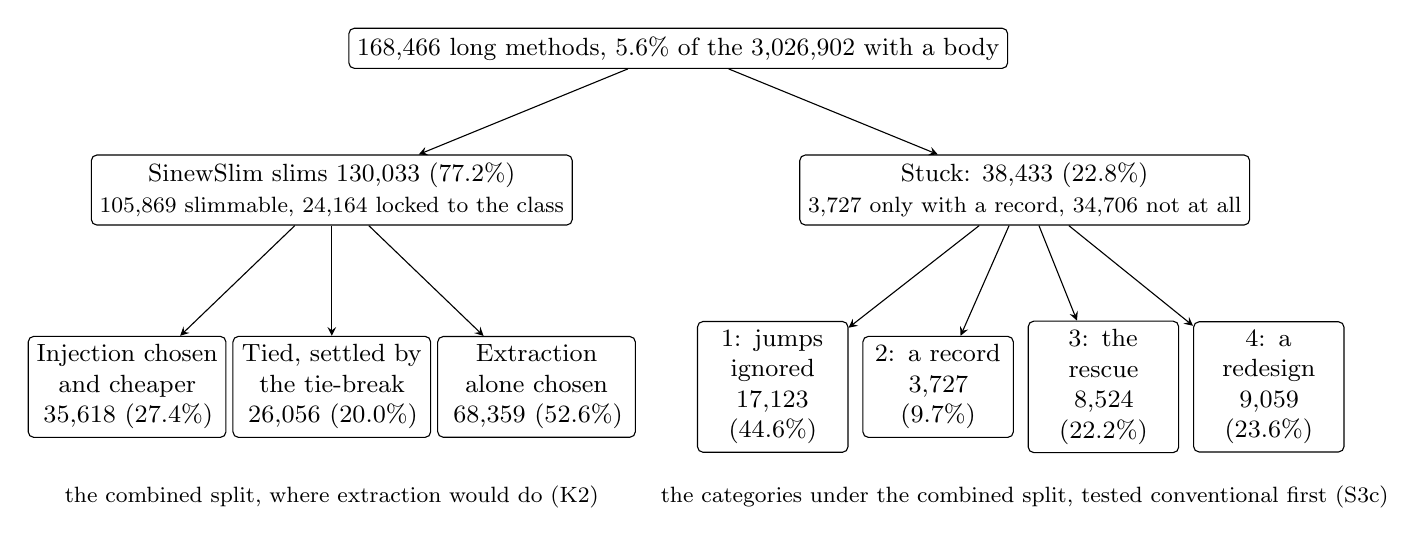
\begin{tikzpicture}[
  every node/.style={font=\small},
  box/.style={draw, rounded corners=2pt, align=center, inner sep=3pt},
  >=stealth]
\node[box] (long) at (0,0) {\nLong{} long methods, \longShare{} of the \nMethods{} with a body};
\node[box] (slims) at (-4.4,-1.8) {SinewSlim slims \nSlims{} (\slimsShare)\\\footnotesize \nSlimmable{} slimmable, \nLocked{} locked to the class};
\node[box] (stuck) at (4.4,-1.8) {Stuck: \nStuck{} (\stuckShare)\\\footnotesize \nRecord{} only with a record, \nNotSlimmable{} not at all};
\node[box, text width=2.3cm] (imp) at (-7.0,-4.3) {Injection chosen and cheaper\\\nImproved{} (\pooledImproved)};
\node[box, text width=2.3cm] (tie) at (-4.4,-4.3) {Tied, settled by the tie-break\\\nTied{} (\pooledTied)};
\node[box, text width=2.3cm] (ext) at (-1.8,-4.3) {Extraction alone chosen\\\nNotImproved{} (\notImprovedShare)};
\node[box, text width=1.7cm] (c1) at (1.2,-4.3) {1: jumps ignored\\\catOneC{} (\catOneCShare)};
\node[box, text width=1.7cm] (c2) at (3.3,-4.3) {2: a record\\\catTwoC{} (\catTwoCShare)};
\node[box, text width=1.7cm] (c3) at (5.4,-4.3) {3: the rescue\\\catThreeC{} (\catThreeCShare)};
\node[box, text width=1.7cm] (c4) at (7.5,-4.3) {4: a redesign\\\catFourC{} (\catFourCShare)};
\draw[->] (long) -- (slims);
\draw[->] (long) -- (stuck);
\foreach \t in {imp,tie,ext} \draw[->] (slims) -- (\t);
\foreach \t in {c1,c2,c3,c4} \draw[->] (stuck) -- (\t);
\node[font=\footnotesize, align=center] at (-4.4,-5.7) {the combined split, where extraction would do (K2)};
\node[font=\footnotesize, align=center] at (4.4,-5.7) {the categories under the combined split, tested conventional first (S3c)};
\end{tikzpicture}}
\caption{The count. Every long method of the \nUsable{} repositories, by SinewSlim's status; the methods it slims, by what the combined split chooses; the stuck methods, by category under the combined split. Shares are pooled over the sample.}
\label{fig:flow}
\end{figure}

\begin{table}[t]
\centering\small
\caption{The long methods by SinewSlim's status, per tier and pooled (L1, L2). The last two statuses are the stuck methods, S1.}
\label{tab:status}
\begin{tabular}{lrrrrr}
\toprule
SinewSlim's status & High & Mid & Low & All & Share \\
\midrule
Methods with a body & 1{,}509{,}345 & 938{,}580 & 578{,}977 & 3{,}026{,}902 & \\
Long (26 code lines or more) & 70{,}918 & 58{,}536 & 39{,}012 & 168{,}466 & 5.6\% of methods \\
\midrule
Slimmable & 44{,}038 & 36{,}010 & 25{,}821 & 105{,}869 & 62.8\% \\
Slimmable, but locked to its class & 10{,}380 & 8{,}913 & 4{,}871 & 24{,}164 & 14.3\% \\
Slimmable only with a record (stuck) & 1{,}467 & 1{,}424 & 836 & 3{,}727 & 2.2\% \\
Not slimmable (stuck) & 15{,}033 & 12{,}189 & 7{,}484 & 34{,}706 & 20.6\% \\
\midrule
Stuck & 16{,}500 & 13{,}613 & 8{,}320 & 38{,}433 & 22.8\% of long \\
\bottomrule
\end{tabular}

\end{table}

\paragraph{The reach, and \Hone{}.} Table~\ref{tab:headline} gives every
headline figure, Table~\ref{tab:headline-tiers} each per tier, and
Table~\ref{tab:categories} the stuck methods by category under each split.
The combined split has a plan for \nStuckPlannedC{} of the \nStuck{} stuck
methods, \ciStuckPlannedC{} of the population, and the injection split alone
for \nStuckPlanned{} (\popStuckPlanned{}). But having a plan is not the
rescue. Tested conventional first, \catOne{} of the stuck methods
(\catOneShare{}) would slim by extraction once their jumps were ignored, and
\catTwo{} (\catTwoShare{}) with a record. What is left is category 3, the
methods only function injection takes apart: \catThreeC{} under the combined
split, \ciCatThreeC{} of the stuck population, and \catThree{} under the
injection split alone. The interval's upper bound, \hiCatThreeC{}\%, lies
below the registered quarter. \textbf{\Hone{} is refuted} by the plan's rule.
The count is far above the minimum of \planHOneMinimum{}; it is the share
that falls short. The median repository's own share, \medianCatThreeC{} over
\reposCatThreeC{} repositories with a stuck method, is lower still, so the
large repositories carry the pooled figure upward, not down. The remaining
\catFourC{} stuck methods (\catFourCShare{}) have no plan from either side.

\begin{table}[t]
\centering\small
\caption{The headline figures (plan, section 6): the count over its denominator, the pooled share, the population estimate weighted by stratum with its \planLevel{} bootstrap interval over repositories within strata, and the median of each repository's own share over the repositories with a method in the denominator.}
\label{tab:headline}
\begin{tabular}{>{\raggedright\arraybackslash}p{4.7cm}rrlrr}
\toprule
Figure & Count / of & Pooled & Population (95\% CI) & Median & Repos. \\
\midrule
Stuck methods the injection split has a plan for & 21{,}329 / 38{,}433 & 55.5\% & 55.5\% (52.0 to 59.0) & 60.0\% & 470 \\
Category 3 under the injection split & 7{,}515 / 38{,}433 & 19.6\% & 19.2\% (17.5 to 21.3) & 14.5\% & 470 \\
Stuck methods the combined split has a plan for & 24{,}327 / 38{,}433 & 63.3\% & 63.3\% (60.1 to 66.5) & 66.7\% & 470 \\
Category 3 under the combined split, the rescue: \textbf{H1} & 8{,}524 / 38{,}433 & 22.2\% & 22.2\% (20.3 to 24.3) & 17.4\% & 470 \\
Improved: injection chosen and cheaper, of what SinewSlim slims: \textbf{H2} & 35{,}618 / 130{,}033 & 27.4\% & 29.0\% (24.3 to 34.6) & 21.5\% & 559 \\
Tied on the sum, settled by the tie-break & 26{,}056 / 130{,}033 & 20.0\% & 20.9\% (19.1 to 23.0) & 19.1\% & 559 \\
\bottomrule
\end{tabular}

\end{table}

\begin{table}[t]
\centering\small
\caption{The headline figures per tier, each pooled within its tier.}
\label{tab:headline-tiers}
\begin{tabular}{>{\raggedright\arraybackslash}p{8.4cm}rrr}
\toprule
Figure & High & Mid & Low \\
\midrule
Stuck methods the injection split has a plan for & 55.5\% & 55.5\% & 55.4\% \\
Category 3 under the injection split & 20.1\% & 19.1\% & 19.2\% \\
Stuck methods the combined split has a plan for & 63.4\% & 63.1\% & 63.4\% \\
Category 3 under the combined split, the rescue: \textbf{H1} & 22.6\% & 21.5\% & 22.4\% \\
Improved: injection chosen and cheaper, of what SinewSlim slims: \textbf{H2} & 27.1\% & 25.8\% & 30.2\% \\
Tied on the sum, settled by the tie-break & 20.2\% & 18.6\% & 21.9\% \\
\bottomrule
\end{tabular}

\end{table}

\begin{table}[t]
\centering\small
\caption{The stuck methods by category (S3, S3c), tested conventional first, under the injection split and under the combined split. Category 3 under the combined split is \Hone{}'s count.}
\label{tab:categories}
\begin{tabular}{>{\raggedright\arraybackslash}p{8.2cm}rrrr}
\toprule
Category of a stuck method & \multicolumn{2}{c}{Injection split} & \multicolumn{2}{c}{Combined split} \\
 & Count & of S1 & Count & of S1 \\
\midrule
1: slims by extraction once its jumps are ignored (conventionally fixable) & 17{,}123 & 44.6\% & 17{,}123 & 44.6\% \\
2: slims by extraction with a record & 3{,}727 & 9.7\% & 3{,}727 & 9.7\% \\
3: a plan under the OfficeFloor column only (the rescue) & 7{,}515 & 19.6\% & 8{,}524 & 22.2\% \\
4: no plan from either (needs a redesign) & 10{,}068 & 26.2\% & 9{,}059 & 23.6\% \\
\midrule
Stuck methods (S1) & 38{,}433 & & 38{,}433 & \\
\bottomrule
\end{tabular}

\end{table}

\paragraph{Where the stuck methods are.} The pooled figure counts each stuck
method once, and the stuck methods are concentrated: Table~\ref{tab:concentration}
gives the ten repositories with the most. The largest, \sig{\topRepo}, holds
\topRepoStuckShare{} of all the stuck methods; the top ten hold
\topTenShare{} and the top thirty \topThirtyShare{}. The median repository
has \medianLongPerRepo{} long methods and \medianStuckPerRepo{} stuck ones;
\reposNoLong{} repositories have no long method and \reposNoStuck{} no stuck
one. Over the \reposCatThreeC{} repositories with a stuck method, the
quartiles of each repository's own rescue share are \catThreeCQone{},
\medianCatThreeC{} and \catThreeCQthree{}: in \reposStuckNoCatThreeShare{}
of them, \reposStuckNoCatThree{} repositories, no stuck method is rescued at
all. The rescue share of the ten largest runs from
\topTenCatThreeCMin{} to \topTenCatThreeCMax{}, around the pooled figure
rather than above it.

\begin{table}[t]
\centering\small
\caption{Where the stuck methods are: the ten repositories with the most, their share of all stuck methods (S1), and the rescue in each under the combined split.}
\label{tab:concentration}
\fitwidth{\begin{tabular}{llrrrrr}
\toprule
Repository & Tier & Long & Stuck & of S1 & Category 3 (combined) & of its stuck \\
\midrule
\texttt{corretto/\allowbreak corretto-8} & Mid & 14{,}560 & 4{,}384 & 11.4\% & 889 & 20.3\% \\
\texttt{OpenLiberty/\allowbreak open-liberty} & Mid & 18{,}374 & 3{,}172 & 8.3\% & 670 & 21.1\% \\
\texttt{apache/\allowbreak hive} & High & 6{,}165 & 1{,}786 & 4.6\% & 360 & 20.2\% \\
\texttt{apache/\allowbreak hadoop} & High & 4{,}907 & 872 & 2.3\% & 165 & 18.9\% \\
\texttt{oracle/\allowbreak coherence} & Low & 2{,}541 & 812 & 2.1\% & 167 & 20.6\% \\
\texttt{elastic/\allowbreak elasticsearch} & High & 5{,}688 & 812 & 2.1\% & 150 & 18.5\% \\
\texttt{openhab/\allowbreak openhab-addons} & Mid & 2{,}821 & 761 & 2.0\% & 212 & 27.9\% \\
\texttt{prestodb/\allowbreak presto} & High & 2{,}121 & 693 & 1.8\% & 235 & 33.9\% \\
\texttt{payara/\allowbreak Payara} & Low & 4{,}373 & 692 & 1.8\% & 124 & 17.9\% \\
\texttt{tranleduy2000/\allowbreak javaide} & Low & 1{,}883 & 628 & 1.6\% & 106 & 16.9\% \\
\bottomrule
\end{tabular}
}
\end{table}

\paragraph{Why the combined split fails.} Table~\ref{tab:reasons} gives
every reason, under each split. A loop longer than the target is the reason
for \loopShareStuckNoPlanC{} of the \nStuckNoPlanC{} stuck methods the
combined split has no plan for: a loop whose body SinewSlim cannot slim
inside the function either. A single statement longer than the target,
usually a \sig{switch} of many short cases, a \sig{try} with resources or a
\sig{finally}, and a \sig{switch} that falls through account for most of the
rest. A jump crossing every cut, the obstacle that most often stops
extraction, stops the combined split on only \jumpsStuckNoPlanC{}: on jumps,
the split does what it was built to do.

\begin{table}[t]
\centering\small
\caption{Why the split has no plan (F1, K1): each reason's count among the stuck methods and among all long methods, under the injection split and under the combined split.}
\label{tab:reasons}
\fitwidth{\begin{tabular}{>{\raggedright\arraybackslash}p{5.4cm}rrrrrr}
\toprule
Reason & \multicolumn{3}{c}{Injection split} & \multicolumn{3}{c}{Combined split} \\
 & Stuck & Share & All long & Stuck & Share & All long \\
\midrule
A loop longer than the target & 8{,}265 & 48.3\% & 18{,}528 & 6{,}133 & 43.5\% & 6{,}133 \\
A single statement longer than the target & 2{,}839 & 16.6\% & 6{,}553 & 2{,}609 & 18.5\% & 2{,}611 \\
A try with resources or a finally & 2{,}491 & 14.6\% & 8{,}544 & 1{,}753 & 12.4\% & 1{,}753 \\
A switch whose cases fall through & 1{,}714 & 10.0\% & 1{,}962 & 1{,}634 & 11.6\% & 1{,}634 \\
More than 5 carried values in every plan & 1{,}618 & 9.5\% & 1{,}921 & 1{,}493 & 10.6\% & 1{,}493 \\
A jump crossing every cut & 177 & 1.0\% & 226 & 484 & 3.4\% & 498 \\
\midrule
Without a plan & 17{,}104 & & 37{,}734 & 14{,}106 & & 14{,}122 \\
\bottomrule
\end{tabular}
}
\end{table}

\paragraph{The shape where both can split.} Where SinewSlim and the
injection split both have a plan, \nBoth{} methods, Table~\ref{tab:shape}
sets the two plans side by side in the terms they share. The injection
split's worst seam is smaller than SinewSlim's widest piece for
\splitSmallerSeam{} of them, equal for \equalSeam{} and larger for
\splitLargerSeam{}; the \nWorse{} methods where it is larger are listed in
the analysis, every one, and \worseByOneShare{} of them are larger by a
single value. Part of that difference is the two definitions rather than the
code: a piece's width counts the method's parameters it reads, and a
function's seam does not, since the framework injects them, so the seam
comparison leans towards the split wherever a method's parameters are read
past the first cut. The scans do not separate the two kinds of value, so how
much of the \splitSmallerSeam{} is definition cannot be read from them; the
reader should take the seam row as a comparison of what each tool prices,
not of two prices of one thing. The injection split makes more parts, more
functions than SinewSlim makes pieces for \splitLargerParts{}, and its
largest function is larger than SinewSlim's largest piece for
\splitLargerLargest{}; both are read with the measure as the plan fixed it,
in which SinewSlim's pieces do not count the remainder and the split's
functions cover every line, so the largest-part row is not a like-for-like
comparison either.

\begin{table}[t]
\centering\small
\caption{Where both SinewSlim and the injection split have a plan (C1, C2): the worst seam, the number of parts and the largest part, with how often the split's is smaller, equal or larger, and the medians. The seam row compares what each tool prices, and the split's seam leaves out the method's parameters where SinewSlim's width counts them; the largest-part row counts the split's functions over every line and SinewSlim's pieces without the remainder, so neither row is like for like.}
\label{tab:shape}
\fitwidth{\begin{tabular}{>{\raggedright\arraybackslash}p{5.6cm}rrrrr}
\toprule
Term & Split smaller & Equal & Split larger & \multicolumn{2}{c}{Median} \\
 & & & & SinewSlim & Split \\
\midrule
Worst seam (C1): SinewSlim's widest piece against the split's most carried values & 70{,}666 (63.3\%) & 35{,}924 (32.2\%) & 4{,}993 (4.5\%) & 2 & 1 \\
Parts (C2): SinewSlim's pieces against the split's functions & 6{,}224 (5.6\%) & 30{,}849 (27.6\%) & 74{,}510 (66.8\%) & 1 & 2 \\
Largest part (C2): SinewSlim's largest piece against the split's largest function & 9{,}389 (8.4\%) & 27{,}622 (24.8\%) & 74{,}572 (66.8\%) & 16 & 24 \\
\bottomrule
\end{tabular}
}
\end{table}

\paragraph{Where extraction would do: \Htwo{}.} Of the \nSlims{} long
methods SinewSlim slims, the combined split chooses injection and costs less
than SinewSlim's cost plus 1 for \nImproved{}: \ciImproved{} of the
population, a median repository share of \medianImproved{}, close to the
\priorImprovedShare{} seen on OfficeFloor's own code before the plan. Another
\nTied{} (\popTied{}) tie on the sum and go to injection by the tie-break,
and \notImprovedShare{} are left to extraction alone. Among the improved
methods the saving is a median of \savingMedian{} (quartiles \savingQone{}
and \savingQthree{}), and \savingOneShare{} of them save exactly 1, so that
their sum equals SinewSlim's cost: the extra function has paid for itself and
no more. That plus 1 is the cost of the method as one function, which a
developer who keeps the method as a method never pays, so the registered
figure is the improvement against extraction inside OfficeFloor. Against
plain extraction, the sum strictly below SinewSlim's cost itself, the share
is \nImprovedStrict{} of the \nSlims{}: \ciImprovedStrict{}, a median
repository share of \medianImprovedStrict{}. The second reading was not
registered; a reader who takes \Htwo{} as ``costs less than extraction''
should take that one.

\paragraph{Post hoc.} Nothing in the four paragraphs that follow was
registered. Each was made after the registered analysis had been read, and
each is a reading of the same scans, not a new measure.

\paragraph{Post hoc 1: the rescue against a narrower denominator.} The
categories credit injection only with what no restructuring could reach, but
the combined split has a plan for \planInCatOneShare{} of the category 1
methods and \planInCatTwoShare{} of category 2, taking them apart as they
stand, with no guard inverted and no record written. Of the
\nNotConventional{} stuck methods that nothing conventional fixes, categories
3 and 4 together, it rescues \rescueOfNotConventional{} (population
\rescueOfNotConventionalCi{}, median repository
\rescueOfNotConventionalMedian{}). The registered reading stands; this one
says where the shortfall against the quarter comes from.

\paragraph{Post hoc 2: test code the scope let through.} The scope's globs
let through test code in directories named otherwise
(\sig{\testTopSegment}, \sig{\testSecondSegment}): \testDroppedLong{} long
methods, \testDroppedLongShare{}, in \testRepos{} repositories. With every
method under a directory whose name contains \emph{test} left out, the
rescue is \testHOneCi{} and \Hone{}'s reading does not change; the
improvement is \testHTwoCi{}. Table~\ref{tab:posthoc-test} gives every
headline figure both ways.

\begin{table}[t]
\centering\small
\caption{Post hoc: the headline figures as registered and with every method under a directory whose name contains \emph{test} left out, each a population estimate with its \planLevel{} interval.}
\label{tab:posthoc-test}
\fitwidth{\begin{tabular}{>{\raggedright\arraybackslash}p{6.2cm}llr}
\toprule
Figure & Registered (95\% CI) & Test paths left out (95\% CI) & Count / of \\
\midrule
Stuck with an injection-split plan (S2 over S1) & 55.5\% (52.0 to 59.0) & 55.1\% (51.8 to 58.2) & 20{,}834 / 37{,}426 \\
Category 3 under the injection split (S3 over S1) & 19.2\% (17.5 to 21.3) & 19.7\% (18.1 to 21.6) & 7{,}426 / 37{,}426 \\
Stuck with a combined-split plan (S2c over S1) & 63.3\% (60.1 to 66.5) & 63.0\% (59.8 to 66.1) & 23{,}749 / 37{,}426 \\
Category 3 under the combined split (S3c over S1): \textbf{H1} & 22.2\% (20.3 to 24.3) & 22.7\% (21.0 to 24.7) & 8{,}425 / 37{,}426 \\
Improved: injection chosen and cheaper, over what SinewSlim slims (K2): \textbf{H2} & 29.0\% (24.3 to 34.6) & 29.5\% (24.8 to 35.1) & 34{,}495 / 122{,}849 \\
Tied on the sum, settled by the tie-break (K2) & 20.9\% (19.1 to 23.0) & 21.0\% (19.2 to 23.0) & 24{,}970 / 122{,}849 \\
\bottomrule
\end{tabular}
}
\end{table}

\paragraph{Post hoc 3: the instrument's faults.} The instrument has one
fault in how it builds a function body's facts, which shows twice. The
combined split has no plan for \nExceptions{} of the \nSlims{} methods
SinewSlim slims (\exceptionsShare{}), which the plan says cannot happen by
construction, \nExceptionsJumps{} of them with the reason \emph{jumps}; and
it has no plan for \nCatThreeLost{} of the \catThree{} methods the injection
split has a plan for, which its outer search contains, all
\nCatThreeLostJumps{} with the reason \emph{jumps}. Both lists are in the
ancillary data and reported to the instrument's project; both count against
injection, and neither touches \Hone{}'s reading.

\paragraph{Post hoc 4: the shape of the plans injection wins.} Every plan
records its functions, each a run, a decision or a handler, and its links,
each a next, a flow or a return, so a plan can be read as a straight sequence
of functions or as branching, with or without early returns
(Table~\ref{tab:shapes}). Where extraction would do and injection is chosen
and cheaper, the plan is a sequence in \shapeImprovedAnySequence{} of the
\shapeNImproved{} methods (\shapeImprovedSequenceReturns{} of them with early
returns), and the tied plans are sequences in \shapeTiedAnySequence{}. Where
injection rescues a stuck method, the plan branches in
\shapeRescuedAnyBranching{} of the \shapeNRescued{}, and
\shapeRescuedSequenceReturns{} are sequences with early returns.

\begin{table}[t]
\centering\small
\caption{Post hoc: the shape of the combined split's plan where it uses injection, read from the plan's functions and links. A sequence has no decision function; early returns are return links from a function other than the last.}
\label{tab:shapes}
\fitwidth{\begin{tabular}{>{\raggedright\arraybackslash}p{5.2cm}rrrrr}
\toprule
Plans & Count & Sequence & Sequence, early returns & Branching & Branching, early returns \\
\midrule
Improved (injection chosen and cheaper) & 35{,}618 & 28{,}252 (79.3\%) & 6{,}088 (17.1\%) & 1{,}062 (3.0\%) & 216 (0.6\%) \\
Tied (chosen by the tie-break) & 26{,}056 & 21{,}644 (83.1\%) & 3{,}807 (14.6\%) & 564 (2.2\%) & 41 (0.2\%) \\
Rescued (category 3, combined split) & 8{,}524 & 2{,}189 (25.7\%) & 852 (10.0\%) & 3{,}849 (45.2\%) & 1{,}634 (19.2\%) \\
\bottomrule
\end{tabular}
}
\end{table}

\section{Discussion}

The author expected function injection to take apart a good share of what
extraction cannot, and set a quarter as the bar. On \nUsable{} repositories
of code written before AI assistants, the registered reading is
\popCatThreeC{}, and the interval excludes the quarter. The expectation was
right in direction against the one repository seen beforehand
(\priorCatThreeShare{} on the framework's own code) and wrong in size against
the bar. A reader sceptical of OfficeFloor should take the figure as it
stands: function injection is not a general fix for stuck methods.

A second reading, not registered, says where the shortfall sits. Nearly half
of the stuck methods (\catOneShare{}) are methods SinewSlim would slim if
their jumps were ignored: the guard-clause and early-return methods. The plan
put them in category 1, conventionally fixable, which was the reading least
favourable to injection and the right one to register, and it stands. What
that category assumes is that ignoring a jump stands for a refactoring a
developer would make. The nearest ones are inverting the guards, threading a
flag through nested \sig{if}s, or extracting the run with a flag the caller
tests and returns on, as an IDE does for one early return; the study prices
none of them, and the first two many would call the worse design. The
combined split handles the jump as it stands, and takes apart three in four
of those methods without restructuring them. Of the stuck methods that
nothing conventional fixes at all, it takes apart about half. That is the
clearest pattern in the data: single-exit extraction, as SinewSlim models it,
cannot deal with an early return, and a flow can. What is left after that,
\catFourCShare{} of the stuck methods, has no plan from either side: loops
whose bodies carry the same jumps and outputs, generated tables, long
\sig{switch} statements of short cases, and \sig{try} blocks with resources
or \sig{finally}. Those are the redesign list, and no split of either kind
shortens it.

The post hoc reading of the plans separates the two results by mechanism,
and the mechanism of the improvement is sequence. Where injection is chosen
over extraction, the method is almost always a pipeline: stages in order,
each consuming what the one before produced, sometimes leaving early.
Extract Method models such a method as a remainder that calls its pieces,
so every stage's product crosses two boundaries, out of the piece that made
it and into the piece that uses it, and the remainder carries all of them.
A sequence of functions models it as what it is: each function hands its
product to the next, priced once, and nothing is carried back to a centre
because there is none. That is what the seam figure measures, and it is why
the improvement is a saving of one or two values rather than more: a
pipeline of a few stages has a few hand-offs. The claim the data supports is
that the long methods people write are often pipelines, and that a pipeline
is cheaper, under the registered cost models, written as a sequence of
functions than contained in a method and lifted into pieces. Whether it is
better written that way is a question about reading, which this study does
not measure; what it measures is that the extraction cost model pays twice
for every hand-off and the flow cost model once. The rescue has the other
mechanism: the methods only injection takes apart are mostly branching, an
\sig{if} or \sig{switch} whose arms become flows,
\shapeRescuedReturnsOfBranching{} of them with early exits, which is where
extraction's single-exit piece fails outright.

The plan defined function injection being cheaper than extraction as its
reach and its shape, never as a comparison of totals. The shape is that,
where both can split a method, the injection split's worst seam carries
fewer values than extraction's widest piece for \splitSmallerSeam{} and more
for \splitLargerSeam{}, with a median worst seam of \medianSplitSeam{}
against \medianSinewSeam{}: what comes from outside the method is injected
and free, which the seam comparison builds in, and what is computed inside
it and carried on is usually one value. It gets there by cutting more.
Whether fewer values in more parts is a better shape is a question about
reading, not one this study measures. Where extraction would do, the
combined split is chosen and cheaper for about three long methods in ten
against extraction wrapped as one function, and for about one in six
against plain extraction, by a median of \savingMedian{}; the saving is
small because the costs are small, and the plan's one-to-one weight between
the two totals decides these choices, so a reader who weighs a flow dearer
than a parameter would see fewer. Every method here was written by people,
before AI coding assistants were in general use; whether code written with
assistants is stuck more often, or in other ways, is a different sample,
and this one gives the baseline it would be compared against.

\section{Threats to validity}

Stuck is relative to the extraction SinewSlim searches: contiguous pieces
with one exit, one output and at most five parameters. An IDE's Extract
Method takes a run with an early return by handing back a flag or an
\sig{Optional} that the caller tests and returns on, and a developer can
write such a piece by hand; SinewSlim does not search that form, so a method
stuck here may come apart under an extraction it does not price. Category 1,
\catOneShare{} of the stuck methods, is where this matters, and the count of
what nothing conventional fixes is a count under one tool's rules. The split
is a projection: none of this code was written for function injection, so a
plan is what the split would cost, not what anyone paid, and the migration
is not analysed here. The injection split's limits decide much: loops and
lambda bodies are never cut between functions, a choice made before the plan
for the framework's own reasons. The seam comparison leans towards the split
by definition, since a function's seam leaves out the method's parameters
and a piece's width counts them; the scans cannot say by how much. The
combined split's tie-break favours injection, so ties are reported apart and
never counted, and its one-to-one weight between the two totals is a choice;
both parts are reported beside the sum, and \Htwo{}'s baseline of SinewSlim's
cost plus 1 includes a function a developer outside OfficeFloor never pays
for, so the reading against SinewSlim's cost itself is reported beside it.
The injection split charges one flow too many for an early return in a
method's last function, as released; it can only overstate that split's
cost. The instrument has the fault of the post hoc paragraph, and a quirk
whereby two runs sharing their first and last lines share one result, left
as it was so that the results would not change between the versions
compared. The scope leaked test code, by the plan's own globs, and the
recount shows the registered figures slightly lowered by it. Generated code
predates AI assistants and is in the sample wherever its directory is not
named \sig{generated}; GUI builders' methods and tables of thousands of
statements are long methods by the definition, stuck, and unsplittable by
either tool. A post hoc lower bound on them: of the \catFourC{} category 4
methods, \catFourGui{} bear a GUI builder's method name and
\catFourLongTable{} are \machineLines{} code lines or more, \catFourMachine{}
together (\catFourMachineShare{}); the longest, \longestMethodLines{} lines,
is a table in \sig{\longestMethodRepo}. The method readings mark
\longOfficeFloor{} long methods as OfficeFloor functions in a sample that
excludes the author's repositories, from another library's
\sig{\ofTopEvidence} annotation; the readings change no cost. Stars measure
attention, not craft, and a repository's tier is its popularity now, not at
the as-of date; a repository deleted or made private since is not in the
frame. The study is Java only, and the author created the framework and
both products: this is why the sample was drawn by a separate tool with a
seed fixed in the plan, why every cost is the products' and fixed before the
plan, why the two totals are never compared, and why every reason the split
fails and every method where it does worse is reported.

\section{Conclusion}

On \nUsable{} open-source Java repositories as they stood before AI coding
assistants, \stuckShare{} of the long methods cannot be slimmed by
single-exit Extract Method as SinewSlim models it. The registered hypothesis
that function injection takes apart at least a quarter of them is refuted:
it takes apart \ciCatThreeC{}. A second reading, not registered, says where
the shortfall sits: nearly half of the stuck methods are early-return
methods the plan counted as conventionally fixable, and the split takes
three in four of those apart as they stand. Of what nothing conventional
fixes, it takes apart about half; about a quarter of the stuck methods need
a redesign that no split provides. Where extraction would do and injection
is chosen instead, the method is a pipeline in \shapeImprovedAnySequence{}
of cases, written more cheaply as a sequence of functions than contained in
a method, because the registered cost models price each hand-off once rather
than twice. The author expected more of the rescue, and the plan was written
so that the data could say so.

\paragraph{Data availability.} Every number here is produced by a script
from the committed analysis, and every table is a generated fragment; the
ancillary data holds the registered plan with its amendments, the sample with
its derivation, the run log, the registered analysis with every
per-repository figure and every method where the split's worst seam is
larger, and the post hoc readings with the methods they list. The raw scans
are reproduced by the study's scripts from the pinned sample and the pinned
jar, so a replication needs no cooperation from the author.

\section*{Competing interests and funding}

The author created OfficeFloor, SinewSlim and OfficeFloorSlim, and has a
commercial interest in OfficeFloor's adoption. No external funding was
received.

\begin{thebibliography}{99}
\small

\bibitem{charalampidou2017} S.~Charalampidou, A.~Ampatzoglou,
  A.~Chatzigeorgiou, A.~Gkortzis and P.~Avgeriou,
  ``Identifying extract method refactoring opportunities based on functional
  relevance,'' \emph{IEEE Transactions on Software Engineering}, vol.~43,
  no.~10, pp.~954--974, 2017.

\bibitem{copilot2021} N.~Friedman,
  ``Introducing GitHub Copilot: your AI pair programmer,''
  The GitHub Blog, 29 June 2021.

\bibitem{fowler1999} M.~Fowler,
  \emph{Refactoring: Improving the Design of Existing Code}. Addison-Wesley,
  1999.

\bibitem{fowler2004} M.~Fowler,
  ``Inversion of control containers and the dependency injection pattern,''
  martinfowler.com, 2004.

\bibitem{haas2016} R.~Haas and B.~Hummel,
  ``Deriving extract method refactoring suggestions for long methods,'' in
  \emph{Software Quality Days (SWQD 2016)}, LNBIP vol.~238, Springer, 2016,
  pp.~144--155.

\bibitem{komondoor2000} R.~Komondoor and S.~Horwitz,
  ``Semantics-preserving procedure extraction,'' in \emph{Proceedings of the
  27th ACM SIGPLAN-SIGACT Symposium on Principles of Programming Languages
  (POPL 2000)}, pp.~155--169.

\bibitem{lanza2006} M.~Lanza and R.~Marinescu,
  \emph{Object-Oriented Metrics in Practice}. Springer, 2006.

\bibitem{maruyama2001} K.~Maruyama,
  ``Automated method-extraction refactoring by using block-based slicing,''
  in \emph{Proceedings of the 2001 Symposium on Software Reusability
  (SSR 2001)}, pp.~31--40.

\bibitem{morrison2010} J.~P.~Morrison,
  \emph{Flow-Based Programming: A New Approach to Application Development},
  2nd ed. CreateSpace, 2010.

\bibitem{longmethod} D.~Sagenschneider,
  ``What reviewers call a Long Method is a length: a pre-registered test of
  coupling divergence as a god-unit signal, and what it settled instead,''
  2026. \url{https://doi.org/10.5281/zenodo.23749773}

\bibitem{silva2014} D.~Silva, R.~Terra and M.~T.~Valente,
  ``Recommending automated extract method refactorings,'' in
  \emph{Proceedings of the 22nd International Conference on Program
  Comprehension (ICPC 2014)}, pp.~146--156.

\bibitem{tsantalis2011} N.~Tsantalis and A.~Chatzigeorgiou,
  ``Identification of extract method refactoring opportunities for the
  decomposition of methods,'' \emph{Journal of Systems and Software},
  vol.~84, no.~10, pp.~1757--1782, 2011.

\bibitem{xu2017} S.~Xu, A.~Sivaraman, S.-C.~Khoo and J.~Xu,
  ``GEMS: an extract method refactoring recommender,'' in \emph{Proceedings
  of the 28th IEEE International Symposium on Software Reliability
  Engineering (ISSRE 2017)}, pp.~24--34.

\end{thebibliography}

\end{document}
